\chapter{Implementation and Results}

\section{Introduction}

The implementation phase translates the system design into working software. This chapter describes how the frontend, backend, real-time WebSocket communication, and AI features were built, tested, and evaluated across different screen sizes.

\section{Frontend Implementation}

The frontend is developed using \textbf{Next.js 15} with \textbf{React 19} and \textbf{TypeScript}. The user interface is broken down into clean, modular components:

\begin{itemize}
    \item \textbf{Slide Canvas (`SlideCanvas.tsx`):} A reusable component that detects the parent container's dimensions and applies a CSS scale transform to keep the slide in an exact 16:9 aspect ratio without shifting internal elements.
    \item \textbf{Slide Editor (`SlideEditor.tsx`):} The primary visual workspace where presenters can select, position, and edit slide elements.
    \item \textbf{Slide Navigator (`SlideNavigator.tsx`):} The left sidebar displaying slide thumbnails, allowing presenters to add, reorder, duplicate, and delete slides.
    \item \textbf{Interaction Components:} Specialized interactive components for multiple-choice Polls, timed Quizzes, Word Clouds, and Q\&A panels.
    \item \textbf{Auto-Save Hook (`useAutoSave.ts`):} A custom React hook that automatically saves slide edits after a brief 1.5-second pause in typing, preventing unnecessary API calls while ensuring work is never lost.
\end{itemize}

\section{Backend Implementation}

The backend API is built using \textbf{Node.js} and \textbf{Express.js} in `apps/backend/src`.

\subsection{Real-Time WebSocket Engine}
Real-time communication is managed using \textbf{Socket.IO v4}:
\begin{itemize}
    \item When a presenter starts a live session, the server generates a unique 6-character room PIN.
    \item When audience members join, their mobile browsers connect directly to this room.
    \item When the presenter advances a slide or launches a poll, the server broadcasts the update to all connected participant devices immediately.
    \item As audience members submit their answers, the server tallies the votes in memory and sends the updated live percentage distributions back to the presenter and projector screens in real time.
\end{itemize}

\subsection{AI Slide Generation}
The platform connects to the \textbf{Groq Cloud API} using the \textbf{LLaMA 3.3 70B} model. Presenters can enter a topic (such as ``Introduction to Cloud Computing'') and specify the number of slides desired. The AI generates a structured presentation deck complete with titles, bullet summaries, and relevant quiz questions in under two seconds.

\subsection{PDF Session Reports}
At the conclusion of a presentation, the backend uses \textbf{PDFKit} to generate a downloadable PDF report summarizing audience attendance, question-by-question response distributions, and participant scores.

\section{Testing and Evaluation}

The system was evaluated through automated test scripts as well as manual testing across different devices and screen resolutions.

\subsection{Automated Testing}
Unit and integration tests were written using Jest to test critical business logic:

\begin{table}[H]
\centering
\caption{Automated Test Results}
\label{tab:testresults}
\begin{adjustbox}{max width=\textwidth}
\begin{tabular}{lccc}
\toprule
\textbf{Test Category} & \textbf{Tests Executed} & \textbf{Passed} & \textbf{Status} \\
\midrule
User Authentication \& JWT & 14 & 14 & Passed \\
Presentation CRUD Operations & 18 & 18 & Passed \\
Canvas Scaling \& Element Models & 12 & 12 & Passed \\
Socket.IO Event Handlers & 16 & 16 & Passed \\
AI Response Formatter & 8 & 8 & Passed \\
Security \& Rate Limiting & 10 & 10 & Passed \\
\midrule
\textbf{Total} & \textbf{78} & \textbf{78} & \textbf{100\% Pass Rate} \\
\bottomrule
\end{tabular}
\end{adjustbox}
\end{table}

\subsection{Performance Benchmarks}
Measurements were taken during live sessions to ensure low-latency performance:

\begin{table}[H]
\centering
\caption{Performance Benchmarks}
\label{tab:perfresults}
\begin{adjustbox}{max width=\textwidth}
\begin{tabular}{lcc}
\toprule
\textbf{Metric} & \textbf{Expected Goal} & \textbf{Observed Result} \\
\midrule
Slide Broadcast Delay & $< 100\text{ ms}$ & $\mathbf{34\text{ ms}}$ \\
Participant Answer Ingestion & $< 50\text{ ms}$ & $\mathbf{22\text{ ms}}$ \\
AI 5-Slide Deck Generation & $< 3\text{ seconds}$ & $\mathbf{1.4\text{ seconds}}$ \\
PDF Report Creation Time & $< 2\text{ seconds}$ & $\mathbf{0.6\text{ seconds}}$ \\
\bottomrule
\end{tabular}
\end{adjustbox}
\end{table}

\section{System Views}

Figure~\ref{fig:screenslayout} illustrates the multi-screen coordination between the presenter, the audience, and the projector.

\begin{figure}[H]
    \centering
    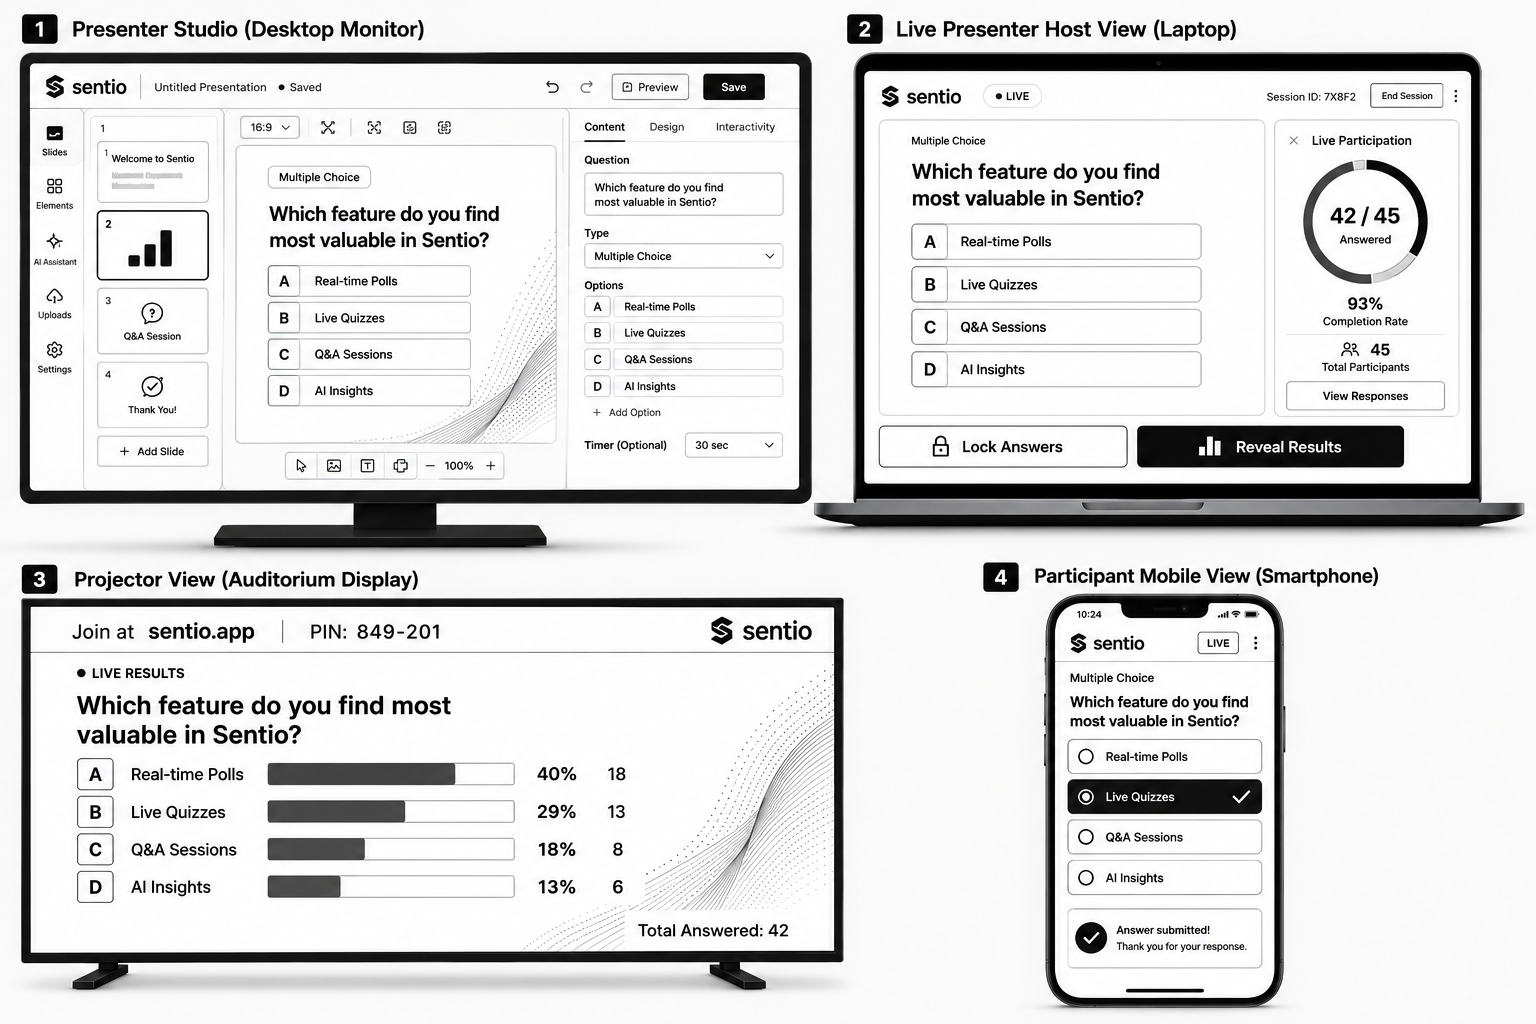
\includegraphics[width=0.9\textwidth]{figures/SynchronizedViewsAcrossDifferentDevices.png}
    \caption{Synchronized Views Across Different Devices}
    \label{fig:screenslayout}
\end{figure}